\documentclass[landscape]{foils} 
\usepackage[pdftex]{graphicx}
\DeclareGraphicsExtensions{.pdf, .jpg, .tif, .png}
%\usepackage{pslatex}
\usepackage{tabularx,dcolumn, graphicx, amsfonts,amsmath}  
\usepackage[sectionbib]{natbib}
\usepackage{picinpar}
\usepackage{paralist}
\usepackage[sectionbib]{natbib}
\bibliographystyle{apalike}
\setlength{\voffset}{-0.5in}
%\setlength{\hoffset}{-0.5in}
%\setlength{\textwidth}{10.5in}
\setlength{\textheight}{7in}
\setlength{\parindent}{0pt}
%\pagestyle{empty}
%\renewcommand{\baselinestretch}{2.0}
\DeclareMathSymbol{\expect}{\mathalpha}{AMSb}{'105}
\def\p{\rm p}
\def\pp{\rm P}
\newcommand{\section}{\secdef \newsection\newsection}
%\renewcommand{\labelitemi}{\includegraphics[width=5mm]{images/bullet.pdf}}
\newcommand{\newsection}[1]{%
{
	\par\flushleft\large\sf\bfseries \vskip -2cm #1\\\rule[0.7\baselineskip]{\textwidth}{0.5mm}\par}}

\newcommand{\subsection}{\secdef \test\test}
\newcommand{\test}[1]{%
	{\par\flushleft\normalsize\sf\bfseries #1: }}
\newcommand{\M}{\mathcal{M}}
\newcommand{\prob}{{\rm Prob~}}
\def\showy#1{{\normalsize\sf\bfseries #1}}
\def\donotuse#1{}

\newcommand{\entrylabel}[1]{\mbox{#1}\hfil}
\newenvironment{entry}
	{\begin{list}{}%
		{\renewcommand{\makelabel}{\entrylabel}%
		\setlength{\labelwidth}{35pt}%
		\setlength{\leftmargin}{\labelwidth+\labelsep}%
	}%
	{\end{list}}}
% this are commands that come with the color package

\usepackage{color}
\usepackage{fancyhdr}


\pagestyle{empty}
%define colors
\definecolor{mediumblue}{rgb}{0.0509,0.35,0.568}
\definecolor{blue}{rgb}{0.0109,0.15,0.468}
\definecolor{black}{rgb}{0.04,0.06,0.2}
\definecolor{darkblue}{rgb}{0.03,0.1,0.2}
\definecolor{darkgreen}{rgb}{0.03,0.5,0.2}
\definecolor{lightblue}{rgb}{0.85,0.9333,0.95}
\definecolor{lightblue2}{rgb}{0.270588, 0.45098, 0.701961}
\definecolor{white}{rgb}{1.0,1.0,1.0}
\definecolor{yellow}{rgb}{0.961,0.972,0.047}
\definecolor{red}{rgb}{0.9,0.1,0.1}
\definecolor{orange}{rgb}{1.0,0.4,0.0}
\definecolor{violet}{rgb}{0.619608, 0.286275, 0.631373}
\definecolor{mybackgroundcolor}{rgb}{1.0,1.0,1.0}

%\definecolor{light}{rgb}{.5,0.5,0.0}
\definecolor{light}{rgb}{.3,0.3,0.3}

% sets backgroundcolor for whole document 
\pagecolor{mybackgroundcolor}
% sets text color
%\color{black}
% see below for an example how to change just a few words
% using \textcolor{color}{text}

\font \riesig=cmssbx10 scaled 13000
\font \gigant=cmssbx10 scaled 12000
\font \gross=cmssbx10 scaled 7000
\font \mittel=cmssbx10 scaled 5000
\font \courier=pcrb scaled 2000

\newcommand{\myFooter}{}
%\begin{picture}(0,0)(0,0)
%	\put(0,-185){\pol}
%\end{picture}}
\newcommand{\myNewSlide}{\newpage\myFooter} % \myBackground}

\usepackage{url}
\usepackage{hyperref}
\hypersetup{backref,  linkcolor=black, citecolor=black, colorlinks=true, hyperindex=true}
\renewcommand{\Pr}{\mathbb{P}}
\usepackage{pdfpages}
\begin{document}

\unitlength=1mm

\begin{center}
{\Large {\bf Likelihood and Bayesian Methods in Biology}}\\
\vskip 5mm

{\large
\url{http://mtholder.github.io/like-bayes-bio/}\par
Mark T. Holder (Univ.~Kansas, USA) \\
\large Thanks to John Kelly and Ford Ballantyne \par
\vskip 1em
HCMR\\
15-18 June, 2015.
}
\end{center}

{
  \normalsize
Source code:\\
   \url{https://github.com/mtholder/like-bayes-bio-4-day-workshop}
}
\myNewSlide
\section*{Goals of the course}
\begin{itemize}
  \item Cover the basic theory associated with point estimation, interval 
  estimation, and hypothesis testing in the maximum likelihood and Bayesian 
  paradigms.
  \item Use some simple computer programs in Python and R to demonstrate that
  it is not too difficult to apply this form of statistical theory.
  \item The examples I use are all ``toy'' simulated datasets, so we will not 
  really get into real biology.
\end{itemize}


\myNewSlide
\section*{Schedule}
\begin{itemize}
  \item Introduction to likelihoods and basic scripts for ML-based confidence intervals (today)
  \item Tuesday:  numerical approaches used to optimize likelihoods, and dealing with multi-parameter models.
  \item Bayesian Introduction: Bayesian inference and Markov chain Monte Carlo
  \item Using model-jumping MCMC to perform model averaging.
\end{itemize}

\myNewSlide
The two competing approaches to statistics:
\begin{compactitem}
  \item frequentist:
  \begin{itemize}
    \item {\bf probability}: the relative frequency of an event if you were able to repeat a trial an infinite number of times.
    \item {\bf goal}: make an argument like ``This result differs significantly from what we would expect if the null model were true. Either the null is not true or we experienced an unusually large amount of sampling error.''
    The $P$-value summarizes how unusual it would be to see results like yours if the null hypothesis were true.
    \item {\bf we make probability statements about}: the long-run performance of our estimation procedures.
  \end{itemize}
  \item Bayesian:
  \begin{itemize}
    \item {\bf probability}: degree of belief
    \item {\bf goal}: express the uncertainty of an estimate:
    ``Given a model and what one knew before one collected the data, one should now believe that the $\Pr(\mu>2.3)\approx 0.87$''
    \item {\bf we make probability statements about}: the true values of parameters/models.
  \end{itemize}
\end{compactitem}

\myNewSlide
\section*{The frequentist ``recipe'' for hypothesis testing}
\begin{compactenum}
  \item Ask a scientific question.
  \item State your question in terms of $H_0$ and $H_A$
  \item Collect a random sample
  \item Calculate a value of a test statistic
  \item Determine $P$-value:
  \begin{compactenum}
    \item What values of the test statistic are expected under $H_0$?
    \item How does the observed test statistic differ from these expectations?
    \item What is the probability of observing a value of a test statistic this extreme or more extreme if the $H_0$ is true? -- this is the $P$-value.
  \end{compactenum}
  \item Make a decision about $H_0$ and $H_A$
  \item Answer your question and report the results.
\end{compactenum}

Choosing a test statistic can be difficult.\\
Deriving a null distribution (step 5a) can be really difficult.
\myNewSlide
\section*{Question: Where does ``likelihood'' fit in?}
{\bf Answer:} the choice of a test statistic in frequentist statistics.
And we'll see that the likelihood is central to Bayesian inference, too.\\

Law of likelihood: ``the extent to which the evidence supports one parameter value or hypothesis against another is equal to the ratio of their likelihoods''
\footnote{definition from \href{https://en.wikipedia.org/wiki/Likelihood_principle\#The\_law\_of\_likelihood}{Wikipedia} -- 
everyone's favorite source of assertions}

Using a likelihood ratio as a test statistic $\rightarrow$ powerful test.

Using maximum likelihood as an estimator: $\rightarrow$ powerful, and statistically consistent (for well-behaved models) estimator.

\myNewSlide
\section*{$P$-values for likelihood ratios}

Sometimes it is analytically tractable to calculate a null distribution.

More commonly, we test null models that are nested within a richer model,
so we use the following trick:

For large sample sizes,\\
if you calculate a likelihood under a model with $x$ extra parameters, \\
2 $\times$ the natural logarithm of\\
the ratio of likelihoods between the larger model and the true model \\
will
be distributed according to $\chi^2_{df=x}$

This is often referred to as the ``likelihood ratio test.''


\myNewSlide
\section*{Definition of likelihood}
In common English usage: ``likelihood'' = ``probability.''

In statistics:
The likelihood of a model/parameter $\theta$ based on observing data $X$ is:
\begin{eqnarray*}
  \ell(\theta) & = & \Pr(X \mid \theta) \\
  \ell(\theta) & = & f(X \mid \theta)
\end{eqnarray*}
Because we use likelihood {\em ratios} for estimation, it is acceptable
to use any function proportional to the probability of the data.
\begin{eqnarray*}
  \ell(\theta) & \propto & \Pr(X \mid \theta) \\
  \ell(\theta) & \propto & f(X \mid \theta)
\end{eqnarray*}

Only compare likelihoods when they are calculated on the same data set $X$.

\myNewSlide
\section*{The sum of likelihoods over all parameter values is$\ldots$}
some number, but nothing you can use.

$$\sum_i \Pr(X \mid \theta_i) \mbox{ is not necssarily } 1$$


By the laws of probability:
$$\sum \Pr(X_i \mid \theta) = 1$$
but we know what our data is, so we do not sum over all possible data sets!

\myNewSlide
\section*{Modeling}
Modeling to perform likelihood calculations is the art of moving from a 
scientific question to abstract representations of the question which
allow you to calculate the probability of a particular data outcome.

Modeling require understanding the rules of probability and often also requires:
\begin{compactitem}
  \item knowledge of what statistical distributions are natural fits for different processes, and
  \item knowledge of some form of stochastic process theory (often Markov processes).
\end{compactitem}
Expertise in modeling requires a lot of training and is beyond the scope of this workshop.

But a few rules, go a long way$\ldots$

\myNewSlide
\section*{rules of probability}
\begin{enumerate}
  \item $\Pr(A) = 1 - \Pr(\mbox{not } A)$
  \item $\Pr(A,B) = \Pr(A)\Pr(B\mid A) = \Pr(B)\Pr(A\mid B)$
  \item $\Pr(A,B) = \Pr(A)\Pr(B)$ if $A$ and $B$ are independent
  \item $\Pr(A\mbox{ or } B) = \Pr(A) + \Pr(B) - \Pr(A,B)$
  \item $\Pr(A\mbox{ or } B) = \Pr(A) + \Pr(B)$ if $A$ and $B$ are mutually exclusive.
  \item $\Pr(A) = \sum_{i=1}^n\left[\Pr(A\mid B=b_i)\Pr(B=b_i)\right]$ if $B \in \{b_1, b_2,\ldots, b_n\}$.
  \item Bayes' rule:$$\Pr(A\mid B) = \frac{\Pr(B\mid A)\Pr(A)}{\Pr(B)}$$
\end{enumerate}

\myNewSlide
\section*{A widely used result from continuous time Markov processes}

If $Q$ is a matrix of instantaneous rates where $q_{ij}$ is the rate
of transitioning from state $i$ to state $j$, then:
$$\Pr(t) = e^{tQ}$$
where $t$ is the time.

This lets us extrapolate about the effects of a constant process over time.

\myNewSlide
\section*{Working some examples}
Now we'll switch to 3 examples.

There is python and R code for 2 of them.

The code is not the most robust in the world - you should try using a number
of optimizers before you publish.

But it should help us demonstrate the concepts.

\myNewSlide
\section*{A toy example: estimating the mean from a sample}
$X$: a set of random, independent continuous measurements sampled from the same population.

Assume that we know the population standard deviation, and want to estimate
    the population mean, $\mu$.\\

\myNewSlide
\begin{eqnarray*}
  \ell(\mu) = \Pr(X \mid \mu, \sigma) & = & \prod_{i=1}^n\Pr(x_i \mid \mu, \sigma) \\
  & = &  \prod_{i=1}^n\left[\frac{1}{\sqrt{2\pi\sigma^2}}\mbox{ }e^{-\frac{\left(x_i-\mu\right)^2}{2\sigma^2}} \right]\\
\end{eqnarray*}
Note that $\mu$ that minimizes the squared error (the least squares estimator) maximizes the likelihood.

\myNewSlide
\begin{eqnarray*}
  \ell(\mu) = \Pr(X \mid \mu, \sigma) & = & \prod_{i=1}^n\Pr(x_i \mid \mu, \sigma) \\
  & = &  \prod_{i=1}^n\frac{1}{\sqrt{2\pi\sigma^2}}\mbox{ }e^{-\frac{\left(x_i-\mu\right)^2}{2\sigma^2}} \\
\log L(\mu)  & = &  \sum_{i=1}^n\log\left[\frac{1}{\sqrt{2\pi\sigma^2}}\mbox{ }e^{-\frac{\left(x_i-\mu\right)^2}{2\sigma^2}}\right] \\
& = &  n \log\left[\frac{1}{\sqrt{2\pi\sigma^2}}\right] + \sum_{i=1}^n\log\left[e^{-\frac{\left(x_i-\mu\right)^2}{2\sigma^2}}\right] \\
& = &  n \log\left[\frac{1}{\sqrt{2\pi\sigma^2}}\right] - \frac{1}{2\sigma^2} \sum_{i=1}^n\left(x_i-\mu\right)^2
\end{eqnarray*}
Note that $\mu$ that minimizes the squared error (the least squares estimator) maximizes the likelihood.

\myNewSlide
\section*{An example from phylogenetics}

If we have a tree $T$ and branch lengths $\nu$ as our model, what is the probability of 
an alignment of DNA sequences?

We can think of a branch length being the product of time $t$ and rate of sequences evolution $\alpha$:
$$\nu = \alpha t$$

\includepdf[pages={20}]{lec11ML.pdf}
\includepdf[pages={16}]{lec10Models.pdf}
\includepdf[pages={25}]{lec10Models.pdf}
\includepdf[pages={21-24}]{lec10Models.pdf}
\includepdf[pages={26}]{lec10Models.pdf}
\myNewSlide
\section*{JC transition probabilities}
$$\Pr_{ii}(\nu) = \Pr(\mbox{end}= i \mid \mbox{start}=i, \nu) = \frac{1}{4} + \frac{3}{4}e^{-4\nu/3}$$

$$\Pr_{ij}(\nu) = \Pr(\mbox{end}= j \mid \mbox{start}=i, \nu) = \frac{1}{4} - \frac{1}{4}e^{-4\nu/3}$$

%\includepdf[pages={19-20}]{lec10Models.pdf}
\includepdf[pages={20-23}]{lec11ML.pdf}

\myNewSlide
\section*{Another toy example}
You tag 1000 territorial animals with transmitting tags.

Every month you survey the area.
Assume that you can detect every tag attached to a living organism.

You know (from other studies) that the probability of a tag falling off are:
0.10 in the first month, 0.15 in the second month, 0.2 in the third month, and
0.25 for every month after that.

Can you estimate the per-month probability of death?

\end{document}
